\section{Cosmological analyses with the \lya\ forest power spectrum}
\label{sec:over}

In this section we present an overview of the different aspects involved in
a cosmological analysis of the small scale clustering from the \lya\ forest
power spectrum.

\begin{itemize}
 \item Measurement of the flux power spectrum: calibrate the quasar spectra,
  fit the quasar continua, measure 2-point functions, estimate covariance
  matrices and assess possible contaminants.
 \item Measurement of the linear power spectrum: using hydrodynamical
  simulations, build an emulator to translate the measured flux power to
  constraints on the linear power spectrum of density at the redshift of
  the measurement ($z \sim 3$).
 \item Cosmological constraints: combine the inferred linear power spectrum
  with external datasets (primarily CMB studies) to constrain the parameters
  of a particular cosmological model.
\end{itemize}


\subsection{Measurement of the flux power spectrum}

\todo{Add here some text on continuum fitting, instrumental noise,
spectrograph resolution, metal contamination...}

\begin{figure}[h]
 \begin{center}
  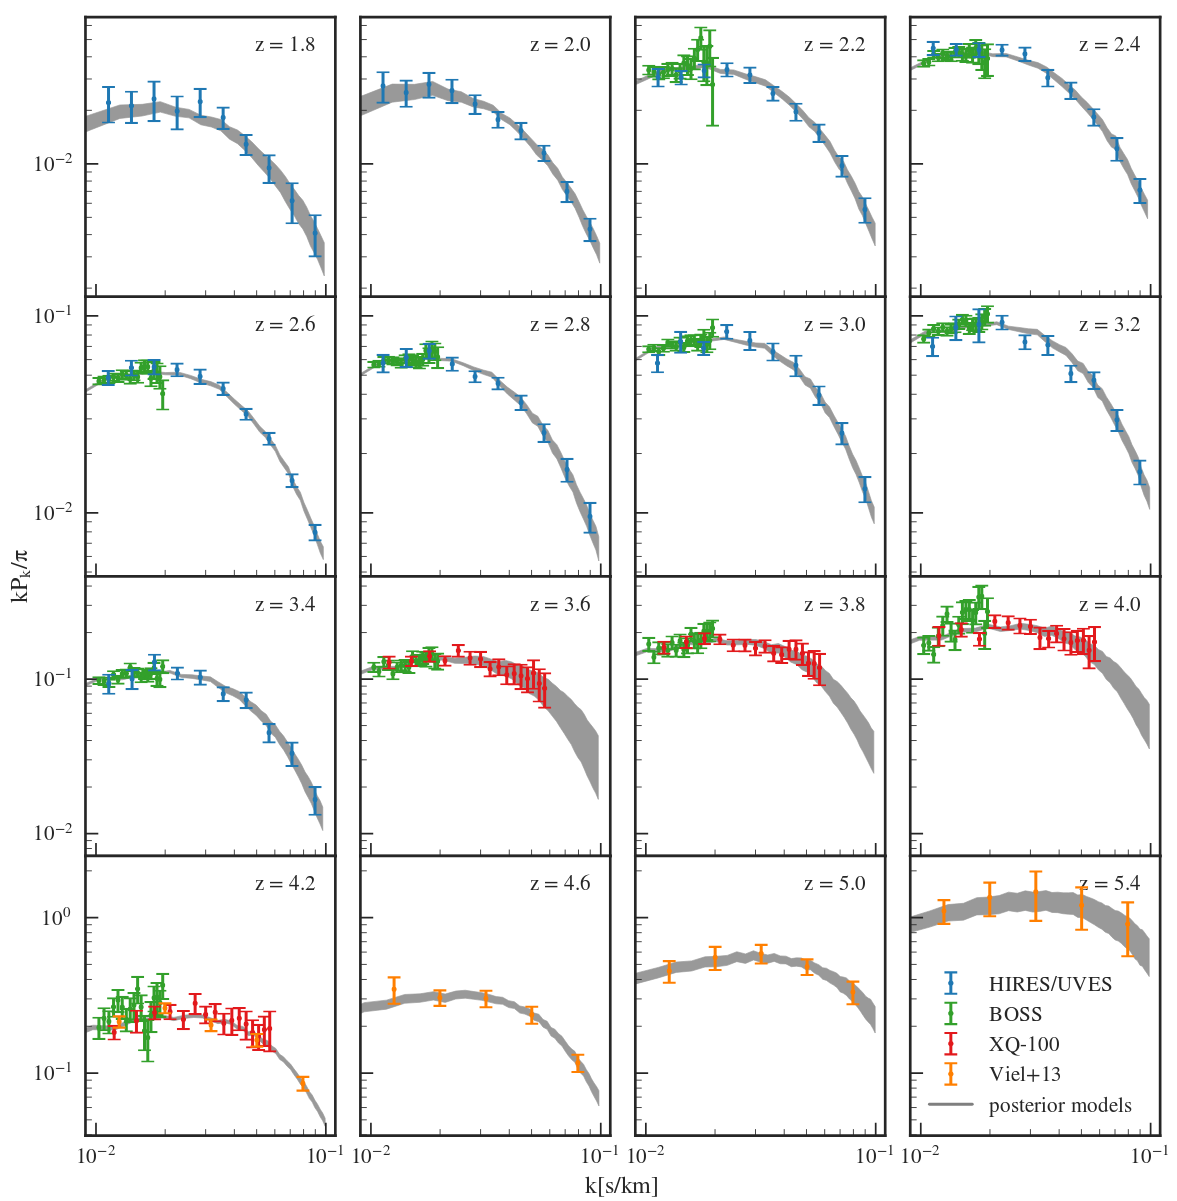
\includegraphics[scale=0.32]{Figures/Walther2018_P1D}
  %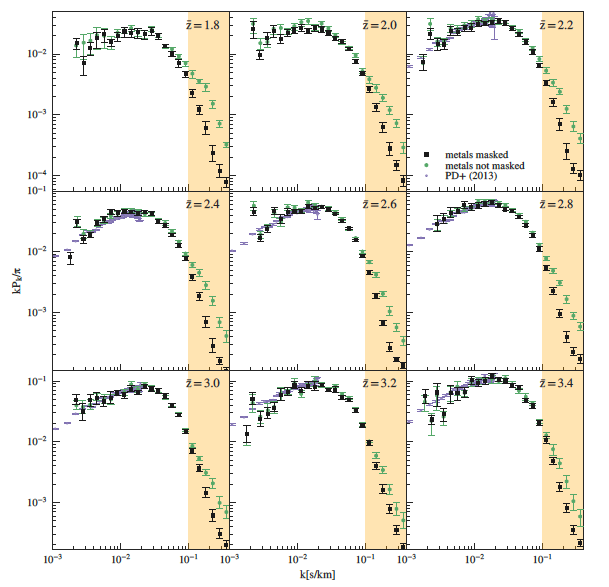
\includegraphics[scale=0.6]{Figures/WaltherP1D}
 \end{center}
 \caption{Compilation of $P_{1D}(z,\kpar)$ measurements, including those from
  \cite{Viel2013} (orange), \cite{Irsic2017} (red), 
  \cite{Palanque-Delabrouille2013} (green) and \cite{Walther2018a} (blue).
  \todo{This figure was stolen from \cite{Walther2018b}, it would be better to
  add one that goes to lower values of $\kpar$ covered by SDSS/BOSS.}
 }
 \label{fig:dataP1D}
\end{figure}

Beyond BAO analyses \cite{Bautista2017,duMasdesBourboux2017}, the only
public results on the clustering of the \lya\ forest are measurements of
the 1D power spectrum \cite{Croft1998,McDonald2000,McDonald2006} or
more recently \cite{Viel2013,Palanque-Delabrouille2013,Irsic2017,Walther2018a}.
These are usually presented as band powers measured in different redshift
bins, spanning the redshift $1.8 < z < 5.4$, and covering a broad range of
scales $0.001 \ikms < \kpar < 0.1 \ikms$.
A compilation of recent measurements is shown in Figure \ref{fig:dataP1D}.

In most cases, the line of sight wavenumbers are expressed in units of
inverse velocity, $\ikms$, but other mappings from observed wavelength
could be used.
When measuring the 3D power, we will also need to define transverse
wavenumbers, and in this case the natural choice will be units of
inverse angles \cite{Font-Ribera2018}.

In the rest of this paper we will assume that the flux power spectrum
has already been measured, and we will focus on its interpretation.
We will mostly discuss the 1D power spectrum, but we will comment on the
differences that one would need to add to apply similar techniques to the
3D power.


\subsection{Measurement of the linear power spectrum}

In order to interpret the measurement of the \lya\ (or flux) power spectrum,
we need to be able to make theoretical predictions, and set up a statistical
method to compare models and compute constraints on their parameters.
Due to its non-linear nature, to model the flux power
spectrum we need to rely on expensive hydrodynamical simulations.
Each model evaluation requires thousands of CPU hours, what makes a
\textit{brute-force} approach unfeasible.

Moreover, the flux power spectrum does not only depend on the density
clustering, but it also depends on the thermal history of the
Inter-Galactic Medium (IGM) (see \cite{Walther2018b} for a recent study).
In order to compute robust cosmological constraints, we need to make sure
that we explore all possible thermal histories, and that we fully marginalize
over these nuisance parameters.
This large parameter space, and the cost of a single run, makes it impossible
to run a simulation for each model we want to compare.
A small number of simulations is usually available, and in the past different
analysis have used different techniques to circumvent this problem:
a smooth dependence was assumed and fit in \cite{McDonald2005a};
a Taylor expansion was used in \cite{Palanque-Delabrouille2013};
a Gaussian Process-based \textit{emulator} was used in
\cite{Walther2018a,Walther2018b}, although in this analysis the cosmological
model was kept fixed and only the thermal history was explored.

Emulators based on Gaussian Processes are an active area of research
\cite{Heitmann2009,Heitmann2014,SLAC2018}, and its application in \lya\
studies is now being studied \cite{Walther2018a,Bird2018,Rogers2018c}.
However, in this publication we will use the term \textit{emulator} in a broad
sense, to describe any setup to use a finite suite of hydrodynamical
simulations to make predictions for the flux power spectrum.

The main topic of this paper is to study the parameter degeneracies in this
type of analyses, and discuss how this might affect the parameterization of
an emulator for the flux power spectrum.

As we will discuss in the next sections, once we have marginalized over
the thermal history of the IGM, the flux power spectrum is mostly
sensitive to the amplitude and slope of the linear power spectrum around
$k \sim 0.01 \ikms$ (roughly $k \sim 1 \iMpc$) around $z \sim 3$
\footnote{As it will be discussed in the next sections, it is convenient
to specify the pivot point in velocity units, since these are the typical
units of the measured flux power.}.
For instance, \cite{McDonald2005a} measured these quantities with 15\% and
5\% precision respectively.

Changes in other (traditional) cosmological parameters are very degenerate
with changes in the linear power or in the thermal history.
For instance, as discussed in \cite{Viel2010} and more recently in
\cite{Pedersen2018}, at fixed linear power spectrum the effect of massive
neutrinos is almost indistinguishable from that of $\Omega_m$.
Another example: at fixed linear power spectrum, and fixed $\Omega_m$, the
effect of $\Omega_b$ is degenerate with the level of UV background assumed.

Another peculiarity of \lya\ forest analyses is that the measurement
covers a redshift range $2 < z < 5$ where the universe was close
to Einsteint-de Sitter (EdS), i.e., $\Omega_m(z) \sim 1$.
This means that the growth of structure in this redshift range is almost
independent of cosmology, and so is the expansion history $H(z)/H_0$.

This approach of emulating only the linear power was used in
\cite{McDonald2005a}, but recent analyses
\cite{Palanque-Delabrouille2015,Yeche2017} have attempted instead to
directly emulate the 6+ traditional parameters of a $\Lambda$-CDM universe.
We will argue that this might not be the best approach, because of the
following reasons:
\begin{itemize}
 \item As discussed above, the traditional parameters have strong degeneracies
  and this makes the emulator (or Taylor expansion) more challenging.
 \item In order to break the degeneracies, one needs to adopt priors from
  CMB experiments, making it more dificult to combine with CMB experiments
  later without double counting information.
 \item The results are model-dependent, and it is impossible to use them in
  extended models (curved universe, non-$\Lambda$, different $N_{\rm eff}$...)
  if these were not in the original emulator.
\end{itemize}


\subsection{Cosmological constraints}

It is only in combination with external datasets, mainly from CMB experiments,
that we are able to provide constraints on the traditional cosmological
parameters.

\begin{figure}[h]
 \begin{center}
  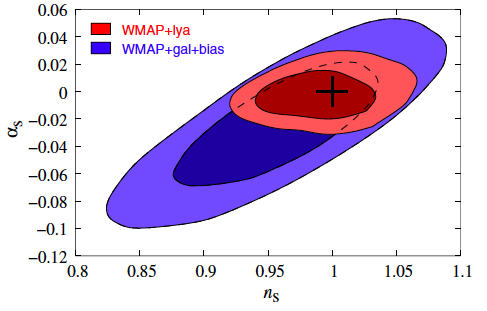
\includegraphics[scale=0.6]{Figures/Seljak2005_contour2D}
 \end{center}
 \caption{Constraints on the shape of the primordial power spectrum of
  perturbations, slope $n_s$ and running $\alpha_s$, from \cite{Seljak2005}.
  The blue contours show the constraints from a joint analysis of WMAP CMB
  data and SDSS galaxy clustering, while the red contours use the same WMAP
  data and the linear power spectrum inferred from the \lya\ analysis of
  \cite{McDonald2005a}.
 }
 \label{fig:Seljak2005}
\end{figure}

For instance, by combining our measurement around $k \sim 1 \iMpc$ with the CMB
constraints on the amplitude and slope of the linear power spectrum at
$k \sim 0.05 \iMpc$ we get tight constraints on the running of the spectral
index ($\alpha_s$) and on the sum of the neutrino masses ($\sum m_\nu$).
This can be seen in Figure \ref{fig:Seljak2005}, copied from \cite{Seljak2005},
where WMAP data was used in combination with the linear power spectrum
inferred from the \lya\ power spectrum \cite{McDonald2005a}.

